\chapter{Evaluation}
The ecosystem of the Bazo cryptocurrency can not be considered completed to a degree where a test run would be possible, at the time of writing. Reasons for this are that the development of the interfaces of the existing infrastructure is not complete. Since these interfaces were specifically designed for the Bazo Wallet during the course of this thesis, the Wallet itself can be considered complete. This chapter assesses the developed Wallet and explains limitations to the system. The assessment of the application is structured into two sections, where the first one focuses on performance aspects and the latter on qualitative metrics.

\section{Quantitative Analysis and Optimization}\label{testing}
In order to assess and optimize the quality of the developed web application in a quantitative manner, Lighthouse was used for the audit. \begin{quote}
Lighthouse is an open-source, automated tool for improving the quality of web pages.
\end{quote}
There exist various work flows to run the tool, however, running it directly from the Google Chrome Developer Tools is suggested by the authors. The audit can be performed against almost any web page and assesses the following five key factors of web applications: \textit{Progressive Web App}, \textit{Performance}, \textit{Accessibility}, \textit{Best Practices} and \textit{SEO}. For each of the metrics, several audits are performed and then summarized to express the scoring as a percentage. It is possible to drill down and obtain detailed information on a failed audit. For some of the audits, the tool can even predict possible enhancements \cite{lighthouse}.
Running the tool against the deployed web application showed the strengths and weaknesses of the implementation. Initially, the application received the full score for \textit{Progressive Web App} and \textit{Accessibility}, which performs audits against the Progressive Web Application Checklist \cite{pwachecklist}. The biggest optimization potential was highlighted through the \textit{Performance} metric, which obtained a result of 44. There were various issues that hindered the performance of the application. These issues and their solution are explained in the following.
\begin{itemize}
\item Render-blocking scripts:

The JavaScript library that contained the decoder for QR-Codes makes up a large part of the application's size. Loading the library from the start of the application had a negative impact on the loading time required until the application is drawn and interactive. This is an interesting fact, since the development of the Shape Detection API, introduced in \ref{qrcodes}, has the intention of avoiding the necessity to include a decoding library in the application. This issue was solved by dynamically loading the library, once the user enters the actual page where the decoding capability is needed.
\item Large images:

Images that are not properly sized can also increase the loading time, thus affecting when the application becomes interactive. The images, supplied by a Design agency were compressed, resized and converted to a more suitable format to decrease the loading and rendering time. By doing so, the size of the assets was decreased by around 80\%.

\item Rendering time:

The time required to render the home page was further optimized by making use of a server-side rendering approach. Since the home page contains mostly static content, it was ideal for this technique. Server-side rendering was achieved by incorporating an optimization plugin into the \textit{webpack}-based build process.
\end{itemize}
The issues described above led to initial loading times of around five to seven seconds until the application becomes responsive. It is important to note that Lighthouse performs these tests under constrained settings. Network speeds are throttled to resemble mobile devices and caching is not leveraged. This testing environment is comparable to a mobile device with a slow network connection accessing the application for the first time. With the performance optimizations described above, the initial loading time was decreased to under two seconds. Subsequent loading times would take around 250ms until the application becomes responsive by leveraging the caching mechanisms.
After optimizing the application, the \textit{Performance} metric received a score of 77.

For the full score of the \textit{Best Practises} metric, the application would have to be deployed to a server that supports HTTP/2. Since this is not part of the actual implementation of the web application and rather a question of deployment, this metric can not be improved with the code basis of the web application.
Lighthouse assesses all audits from the user's computer. This might impact the validity of the Performance audit. Although this audit is already performed with a constrained network to simulate mobile environments, the audit could suffer from other impacting factors. For this reason, another popular performance testing service, Pingdom, was used to verify the results. Pingdom differs from Lighthouse in such a way that it runs the tests from a server, where an intercontinental grid of servers is used to determine the performance of the application \cite{pingdom}. The Bazo Wallet was tested from all the locations available in the tool and consistently obtained the highest performance grade. Figure \ref{fig:pingdom} summarizes a performance audit with Pingdom for one location.
\begin{figure}
\centering
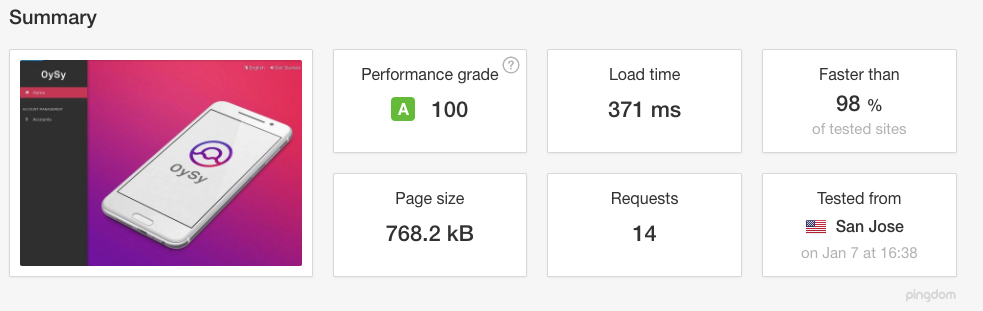
\includegraphics[width=1\textwidth]{screenshots/pingdom.png}
\caption{\label{fig:pingdom}Summary of a Performance report using Pingdom.}
\end{figure}

Lighthouse specifically advises to conduct manual checks to ensure an appropriate user experience on multiple browsers and platforms. The same strategy is proposed for testing User Interfaces, with regard to page transitions and animations. 
Since the complete functionality with all branches can be tested relatively quickly, the complete app was tested for a variety of devices. The rest of this chapter gives insight into the testing results and the tested combinations of operating systems and browsers.


\begin{center}
    \begin{tabular}{ | l | l | l | l | p{2cm} |}
    \hline
      & Internet Explorer & Google Chrome & Safari & Firefox \\ \hline
    macOS X (10.12.6)  & no (deprecated) & yes & yes & yes \\ \hline
    Windows 10 (14393.479)  & yes & yes & no (deprecated) & yes \\ \hline    
    iOS (11.1.2)  & no (not available) & no & yes & yes \\ \hline
    Android (8.0.0)  & no (not available) & yes & no (not available) & yes \\ \hline
    \end{tabular}
    \captionof{table}{Overview of tested browsers and operating systems.}\label{table:testing}
    \end{center}
Table \ref{table:testing} shows targeted platforms where the complete functionality of the Bazo Wallet was tested. The web application proved to work as expected from the evaluation of cross-browser support for the leveraged APIs as described in \ref{browsersupport}. Testing the web application in Safari on an iOS device revealed that there are still several issues with PWAs on iOS; The application behaves differently, depending on if it is run directly from Safari or from the home screen. Given that WebKit, the browser engine used by Safari, still does not completely support PWAs explains the lack of stability. Many of the technologies used with PWAs, such as Service Workers, are not completely implemented at the time of writing \cite{webkitsw}. However, using the web application in Safari provided a consistent user experience. All elements that require unsupported features were hidden from the user.
 
All parts of the application that contain interaction with the Bazo network can be considered critical functionality. The same applies to other parts which are important for the security of a user's funds. In order to simplify testing and improve reusability, all of these operations were bundled into a JavaScript library. Hence, this library consists of methods that wrap the web interface of the Bazo client, outlined in \ref{bazoclientwebinterface}. The library further contains helper functions for operations, such as generating appropriate key pairs. The Bazo Wallet only needs to be able to create one of the three types of transactions that are possible within Bazo. However, to promote the library's reusability, the scope of the library was extended for all transaction types and their respective helper methods.
The library was tested using the \textit{mocha} testing framework in conjunction with \textit{istanbul} for code coverage analysis. 97.5\% of all lines were covered by the unit tests, see Figure \ref{fig:coverage}. Modularizing all payment related operations into a library further allows assessing the speed of a payment with the Wallet. The helper method of the JavaScript library, which allows to prepare, sign and distribute a transaction, was tested under constrained network access to simulate a mobile environment. Running the tests iteratively revealed a consistent performance for the operation, which took between 1500 and 2000 milliseconds. The duration of the operation can be explained by looking at the implementation, which consists of three synchronous http requests and the computation of the transaction's signature. Each request had an impact of around 500 to 600 milliseconds to the operation. The unit tests of individual methods running the same requests on their own showed similar performance. Computing the transaction's signature showed a performance impact of around 10 milliseconds. This result is comparable to the results of the benchmarking performed by the maintainer of the utilized JavaScript library \cite{elliptic}. 
Since most of the time for the operation is lost while connecting to remote systems, the mobile port of the Bazo client, described in \ref{futurework}, could dramatically improve the performance of this operation.

\begin{figure}
\centering
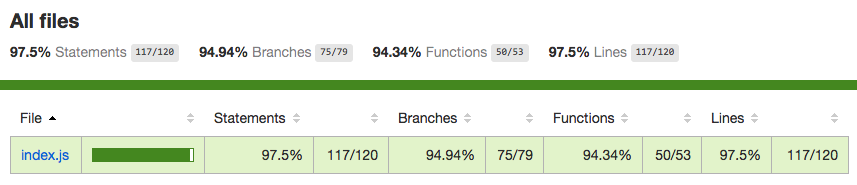
\includegraphics[width=1\textwidth]{screenshots/bazo-api-testing.png}
\caption{\label{fig:coverage}Coverage report of the Bazo API library.}
\end{figure}
\section{Qualitative Evaluation}
This section evaluates the developed P2P mobile payment application against key characteristics for such a solution. Qualitative Key characteristics of a mobile payment solution can be:
\begin{enumerate}
\item \textbf{Payer control}
The degree as where a user can select the most advantageous terms for his payment.
\item \textbf{Security}
The degree of risk of having funds manipulated or stolen by engaging in the payment system is considered Security.
%inverse?%
\item \textbf{Universality}
This key characteristic deals with the importance of a payment system being accepted by a large user base to make the payment solution attractive.
\end{enumerate}

Payer control with the Bazo currency has a mixed image.
The user has the control to create transactions at terms he prefers, for example, the user can set the fee he is ready to spend for the transaction. However, the clearance of the transaction highly depends on the network. That is the current amount of unconfirmed transactions, the rate at which transactions are validated and the fee the user has set. The user has little to no influence on these conditions.

Security, as in the definition above, should be given for all transactions signed by the user. Section \ref{limitations} outlines cases, where the user can be tricked to reveal his public key. From a technical point of view, the Wallet can be considered secure, as that it is not possible to steal a private key or manipulate transactions which would result in the loss of funds for the user.

Universality is not a strength of the Bazo currency. Since the Wallet is not compatible with other payment systems or applications, only users in the system can exchange funds. Since Bazo is a newly created cryptocurrency, there is no user base and users would have to be convinced to join the system. Given that the target users should already be in the bonus program, the usage of the Bazo currency could be offered an incentive. Since the mechanisms in the Wallet for communicating with the currency are very similar to the mechanisms in other currencies such as Ripple, it would technically be feasible to reuse the Wallet for other currencies and map the bonus points to said currency \cite{ripplelib}, thus leveraging an existing user base.

\section{Limitations}\label{limitations}
This chapter introduces limitations of the developed systems and how they can be improved.
\begin{itemize}
\item \textbf{Trust} 
It is an objective of many cryptocurrencies to be as independent from third parties as possible. This should that assets can be traded in a trustless way. Since, the application is designed as a signing-only client, there needs to exist a certain amount of trust between the user of such a Wallet and the server he relies on \cite{bitcoinclients}. With this architecture, it is technically possible to tamper with the information that is sent to the client, such as account balances. This is due to the client being unable to verify the transactions in the same manner that other applications can. However, it is not possible to modify outbound transactions and thus steal assets from the user of the developed system.
This is ensured by having all transaction signing implemented in the browser. Since sharing transaction data is not performed over the same server, but rather on a P2P basis, it is also hard to trick the user into targeting the wrong address.
Another solution to further reduce this threat is giving users the freedom to connect to a specific server. In the Bazo Wallet, the user has the possibility to set a URL on the \textit{Settings} Page. This URL is persisted locally and used for all further communication. That way, users could deploy the light client to an https enabled server and use this node as a private backend. This approach is frequently employed when dealing with signing-only clients \cite{bitcoinclients}. It is also technically possible to run the light client locally on an android phone, by running the binaries of the light client. This was tested and proven to work as with any other operating system or platform.
\item \textbf{Phishing} 
Another risk is introduced with the unified data model of transaction data, since this points to the URL of the Bazo Wallet. One could trick a user into using a web application that looks like the Bazo Wallet, but has the single purpose of stealing the private key. This is a serious risk in cases where the user does not realize that the URI does not belong to the actual Wallet.
One solution how this weakness can be handled is to install the progressive web application to the home screen. On Android systems, this will associate the installed application with the URI of the origin. Therefore, the application will only open if the host of the URI matches the origin of the installed web page.
\item \textbf{Browser Support} 
Chapter \ref{transactoinsharing} assessed the support of different operating systems for new, web-based APIs. Especially Safari on iOS devices lacks many of the newer features. These inconsistencies between browsers were handled with a Progressive approach, where the User Interface only shows the available transferral types. For every device, a fallback solution ensures that there is some way of transferring transaction data.
This limitation is unfavorable since the financial service provider estimates the majority of potential users to use an iOS device. Because of this, the development of a native iOS application, that would wrap the web application, is being discussed. However, the assessment of the technical feasibility and the actual implementation are not part of the scope of this thesis.

\end{itemize}

\newpage

\chapter{Future Work}\label{futurework}
During the development of the Bazo Wallet, limitations with respect to the current implementation of applications in the Bazo ecosystem were observed. This chapter summarizes the issues and possible solutions.

\section{Web-based Headers-only Client}
Chapter \ref{requirementsanalysis} contained an analysis of the application that was to be developed. Due to the elicited requirements and the design guidelines the application was developed as a signing-only client. Considering only the resources available to such an application, it would be possible to develop a headers-only client for a blockchain based currency. For the Bazo currency, this was not applicable for two reasons. Firstly, a web application can not participate in the peer-to-peer network over a TCP connection. Secondly, a solution for using JavaScript or a similar mechanism to validate blocks would need to be found. The first of these issues could be solved by implementing a web service that allows a web application to download block headers over an https or wss connection. This web service could be in the form of a standalone application or integrated into the RESTful API of the Bazo Light client.%% The second issue would have to be solved by changing the way that transactions are signed and verified. The necessary changes would require a change of the protocol. This would imply a fork of the blockchain for a productive system.

\section{Native Mobile Client}
Chapter \ref{bazomobile} proved that it is technically possible to run the bazo client and even the bazo miner application on a mobile device running Android. This was done with the intention to allow the PWA to communicate with a trustable Bazo node. The necessity of this solution lies in the weakness of signing-only clients which rely on a web service and thus on a third-party. To allow a user to use the compiled binaries in a comfortable manner, the following issues would have to be evaluated and solved:
\begin{itemize}
\item Android wrapper application:

The compiled binaries of the PoC can be run from the command line. However, an android application that would wrap and run the binaries would need to be developed.
\item Communication between native and web application:

Most of the communication between the two applications could be achieved through the RESTful API. However, running the two applications consistently would possibly require extension of the API. Another way how these types of applications can exchange data based on user input is through the intent system. This approach was also proved to work in the NFC Bridge application, see \ref{nfcbridge}, and might be a more resilient channel of communication.
\item Network constraints:

Chapter \ref{bazomobile} outlined constraints posed on a PWA. This would imply for the PWA to establish a secure connection to the native application. Depending on the way how the two applications communicate, this could involve further efforts, such as enabling the native application with https.
\end{itemize}


\section{Integrating Third-Party services}

Chapter \ref{merchantoptions} and \ref{onboarding} introduced two processes dependent on interfaces and applications on the side of the financial service provider. The mechanisms, processes and interfaces required in the company's infrastructure were designed in partnership. All necessary operations in the Wallet have been implemented. At the time of writing, the necessary developments on the company's side have not yet been completed. This means that minor adjustments to the code base of the PWA, such as setting an URL for the submissions, are needed in the future. In order to simplify the development of the application required in the company's backend, the scope of the Bazo API library was extended for the transaction types that will be needed in the onboarding process. Thus, the developers on the company's side, have two possibilities to execute the required functionality on the Bazo network. It is possible to run the operation directly by running the binary as a subprocess, or through the web API. If the latter approach is chosen, it is possible to make plain http requests to the API or reuse the Bazo JavaScript API.
\newpage
